\chapter{Description générale}

\section{Environnement du projet}
Pour ce projet, je me base sur le code de mon encadrant, qui résout le sous-problème où l'ordre de réalisation des jobs et la constitution des lots sont fixées.
Le code est écris en C++ avec Visual studio 2017 et utilise la bibliothèque Cplex.

Le projet existant utilise des fonctionnalité de Visual c++ et n'est pas compatible avec le C++ standard,
 une partie de mon travail consiste à l'adapter.
\section{Caractéristiques des utilisateurs}
Il s'agit d'un projet de recherche, les utilisateurs seront des chercheurs souhaitant tester les algorithmes développé dans ce projet.
 
\section{Fonctionnalités du système}
L'application développé dans ce projet à pour objectif de trouver la meilleur solution pour le problème définit précédemment.
Elle est utilisé pour comparer les résultats des différents algorithmes.
Deux méthode sont exploré, une méthode exacte utilisant un solveur et l'autre une méthode heuristique.

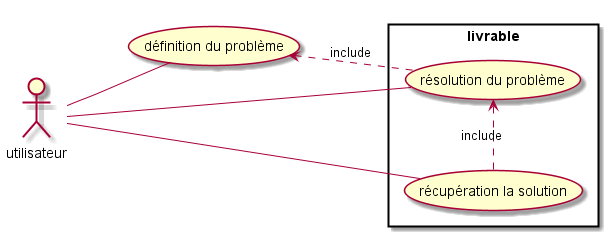
\includegraphics[width=\textwidth]{parts/description_generale/use_cases}
\section{Structure générale du système}

Le programme comprendra une partie commune pour les deux algorithmes.
Cette partie commune comprendra :
\begin{itemize}
    \item les descriptions des instances.
    \item les descriptions des solutions.
    \item les validations des solutions.
\end{itemize}

L'utilisateur pourra choisir la méthode a utiliser.